\renewcommand{\theequation}{\theenumi}
\begin{enumerate}[label=\arabic*.,ref=\thesubsection.\theenumi]
\numberwithin{equation}{enumi}

\item Let +x axis be east and +y be north direction. Also let $\vec{v_b}$ and $\vec{v_w}$ represent the velocity of boat and wind respectively along. 
\item Then 
\begin{align}
\vec{v_w} &= \myvec{72\cos45\degree\\72\sin45\degree} \\
\vec{v_b} &= \myvec{0\\51}
\end{align} 
\item The direction of the flag on the boat will be the relative velocity of wind w.r.t boat. So let $\vec{v_{wb}}$ represent the direction of flag. Then
\begin{align}
\vec{v_{wb}} &= \vec{v_w}-\vec{v_b} \\
&= \myvec{36\sqrt{2}\\36\sqrt{2}-51} &= \myvec{50.91\\-0.09}
\end{align}
\item Let the angle made by $\vec{v_{wb}}$ w.r.t x-axis(east) be $\alpha$. Then
\begin{align}
\alpha &= \tan\brak{\frac{-0.09}{50.91}}\\
&= -0.1\degree
\end{align}
\item The direction of flag on the boat is 0.1\degree w.r.t east.

\begin{figure}[!ht]
\centering
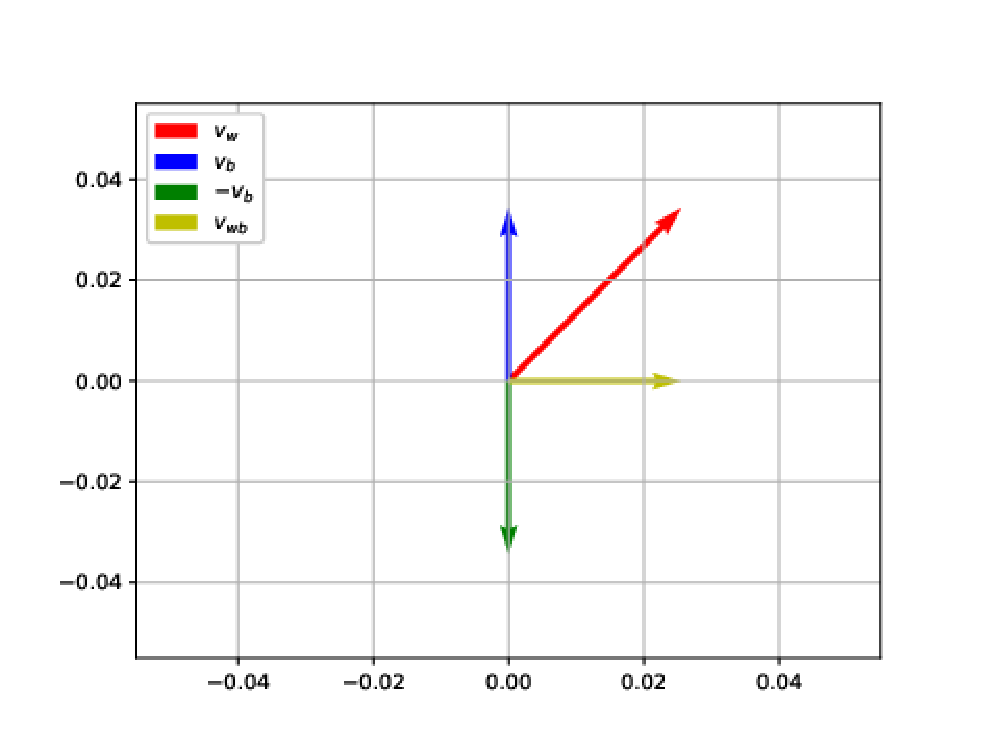
\includegraphics[width= \columnwidth]{./figs/line/motion/motion.eps}
\caption{Vectors representing different velocities}
\end{figure}
\item The python code for the figure can be downloaded from
\begin{lstlisting}
codes/line/motion/motion.py
\end{lstlisting}

\end{enumerate}